\documentclass[conference]{IEEEtran}
\IEEEoverridecommandlockouts
% The preceding line is only needed to identify funding in the first footnote. If that is unneeded, please comment it out.
\usepackage{cite}
\usepackage{amsmath,amssymb,amsfonts}
\usepackage{algorithmic}
\usepackage{graphicx}
\usepackage{textcomp}
\usepackage{latexsym}
\usepackage{xcolor}
\def\BibTeX{{\rm B\kern-.05em{\sc i\kern-.025em b}\kern-.08em
    T\kern-.1667em\lower.7ex\hbox{E}\kern-.125emX}}
\begin{document}

\title{Obstacle Tower Challenge}

\author{%
  \makebox[.5\linewidth]{Aditya Chandupatla}\\University of Southern California\\ Los Angeles, CA \\chandupa@usc.edu\\
  \and \makebox[.5\linewidth]{Avantika Shenoy}\\University of Southern California\\Los Angeles, CA \\avantika@usc.edu\\
  \and \makebox[.5\linewidth]{Hardik Surana}\\University of Southern California\\Los Angeles, CA \\hsurana@usc.edu\\
  \and \makebox[.5\linewidth]{Pranshu Dave}\\University of Southern California\\Los Angeles, CA \\pranshur@usc.edu\\
}

\maketitle

\begin{abstract}
Obstacle Tower Challenge is a procedurally generated environment where the player's goal is to climb as many floors of the tower before time runs out. To tackle this challenge, the following problems must be solved: the vision system for the agent, the three dimensional spatial movement-based skills of the agent, planning on an abstract level, and generalizing the decision-making process. The paper proposes reinforcement learning based approaches to solve these problems. In particular, it investigates use of different algorithms, namely policy gradients and proximal policy optimization for this purpose. For smoother training, A3C architecture with thread-based parallelism for these algorithms is used. Future work will involve testing the efficacy of curiosity driven learning and use distributed training using distributed tensorflow and IMPALA.
\end{abstract}

\begin{IEEEkeywords}
Reinforcement learning, Asynchronous Advantage Actor-Critic (A3C), Proximal Policy Optimization (PPO), Importance Weighted Actor Learner Architecture (IMPALA)
\end{IEEEkeywords}

\section{Introduction}
Regardless of the improvements and progress made in instrumenting new algorithms, most scientists are still focusing on arcane methods of playing games such as Breakout and other similar games. The issue with these games is that the graphics involved are pretty rudimentary, and easy to predict. The algorithms might as well overfit to the game and mark it as solved. Therefore they are uninteresting and not fruitful.

Given these drawbacks, Unity developed a procedurally generated environment called the Obstacle Tower Challenge \cite{Juliani-et-al} that would serve as an interesting tool which can be used as a yardstick to measure the progress made in contemporary artificial intelligence algorithms in reinforcement learning to their limits. Currently, the focus is on the agent's computer vision capabilities, locomotion skills, abstract thinking, and the way they generalize. Better agents means better non-player-characters, thorough testing, and finally more engaging player experiences.

Arcade Learning Environment (ALE) is one of the most sought after game environments used in reinforcement learning research \cite{Bellemare-et-al}\cite{Mnih-2015} so far. Such games are two-dimensional, have low-pixel graphics resolutions, operate in a fixed layout, have limited branching factors and do not require agents to be trained for generalization.

The Obstacle Tower Challenge game is a complete overhaul of its predecessor, the ALE. It is a high-fidelity game that operates in 3D, generates new visuals and themed layouts with each level and game using "Procedural Content Generation", has a high branching factor and requires agents to learn to solve sub-tasks. Although this game is more advanced than before, this adds those many challenges to develop agents that can match human level performance. RL researchers are focusing on developing autonomous agents that can perceive more information, strategize as well as control low-level actions to achieve high scores in this game.

The goal of this project is to develop and train an AI agent using state-of-the-art reinforcement learning techniques that can successfully maneuver the OTC game and solve an above-average number of levels. This project will also help the authors gain hands-on knowledge about generalization in AI and its challenges.

The rest of this paper is structured in the following way. It starts with a discussion of past approaches to solving the challenge and how each of them fared. It then dives into environment characteristics. The next part discusses current progress in methods used to solve the challenge and the final two sections discuss results and limitations.

\section{Related Works}

Since this game is relatively new, our literature survey around the game and model approaches are focused around techniques used by other participants of the challenge.

Gianni et al. \cite{Unity-tech-blog} investigated the use of KL-divergence terms for behavioral cloning for initial levels, but due to poor results in later levels dropped the idea. They also tried training an agent by using world models but that didn't work too. They then used a reduced action space and reshaped their reward function to boost training time. They used PPO to train the agent on these updated parameters. This method worked well and helped them place second in the final challenge. 

Songbin \cite{Unity-tech-blog} used PPO + behavioral cloning for training the agent. He used the PPO version implemented in the ML-Agents toolkit and used a replay buffer for incorporating human play in training. The NN model he used included a gated recurrent unit (GRU) to help the agent learn temporal dependencies of actions. Some other tricks that were used in the NN were Dropout, data augmentation and different sequence lengths. His top scoring agent was able to achieve high floors in the high 20s. 

The winner, Alex \cite{Pickled-ml-blog} made use of two agents. One that solved levels 1-9 and the other solved level 10 onwards. The agent that solved level 10 and above was trained with floors from 10-15. The Sokoban puzzle problem was immediately solved as a result of this since the agent did not have to spend time solving the first ten floors and could focus on the puzzle alone.

To make it easy to play the game as a human, a reduced action space was introduced.  The CNN architecture from IMPALA was used since it is known to have performed better in terms of generalization. By rescaling a standard initialization, the Fixup initialization \cite{Zhang-et-al} solves the problem of vanishing gradient. Residual networks were also trained with Fixup and were found to be equally stable. The state classifier was trained with fewer labeled examples by using MixMatch. \cite{Berthelot}

Data augmentation was used in two scenarios by Alex: for behavior cloning by using traditional image data and during "prierarchy" training. With the use of mirroring data augmentation, which essentially means images and actions were imitated together, the quantity of training levels were doubled as each level had a mirror image associated with it. To resolve the problem of overfitting, data augmentation was used on the environment while training the agent with "prierarchy". 


\section{Environment}
The game is developed by Unity using the ML Agents \cite{Unity_ml_agents_tech_blog} toolkit. An OpenAI Gym \cite{Open-ai-gym} wrapper has also been created to standardize the environment and allow users to implement multiple RL algorithms. 

The game begins with the player at the entrance of the first floor of a tower with a timer of 30 seconds. The player must move around the floor and cross doors to reach the next floor. The player can continue to play the game until the timer drops down to zero. The player can perceive the state it is in and is also given information such as which floor it is currently on, the number of keys it possesses and the remaining time. 

With each increasing floor level, the complexity of crossing it increases. The player will face challenges such as decreasing time, larger floor maps, locked doors (for which it must find and acquire a key), and puzzles like Sokoban \cite{Sokoban} that must be solved. 

To help the player, time orbs have been placed at random locations that add 5 seconds to the timer. The player is also incentivized when it crosses doors, solves any of the above-mentioned sub-tasks and crosses a floor/level using a dense reward system. 


\section{Methods (Software and Algorithms)}

The project follows a typical reinforcement learning framework. As seen in Fig. \ref{gameplay_setup}, the observation is first collected from the environment. This includes the state image, number of keys in possession, remaining time and the current floor the player is on. We then process the state, which comprises of an RGB image of (84 * 84 * 3) dimensions by passing it to the model which is built using the Actor-Critic setup. The model extracts features, parses temporal dependencies and gives a softmax probability distribution of actions. We then select the action with highest probability and simulate the action in the environment.

\begin{figure*}
  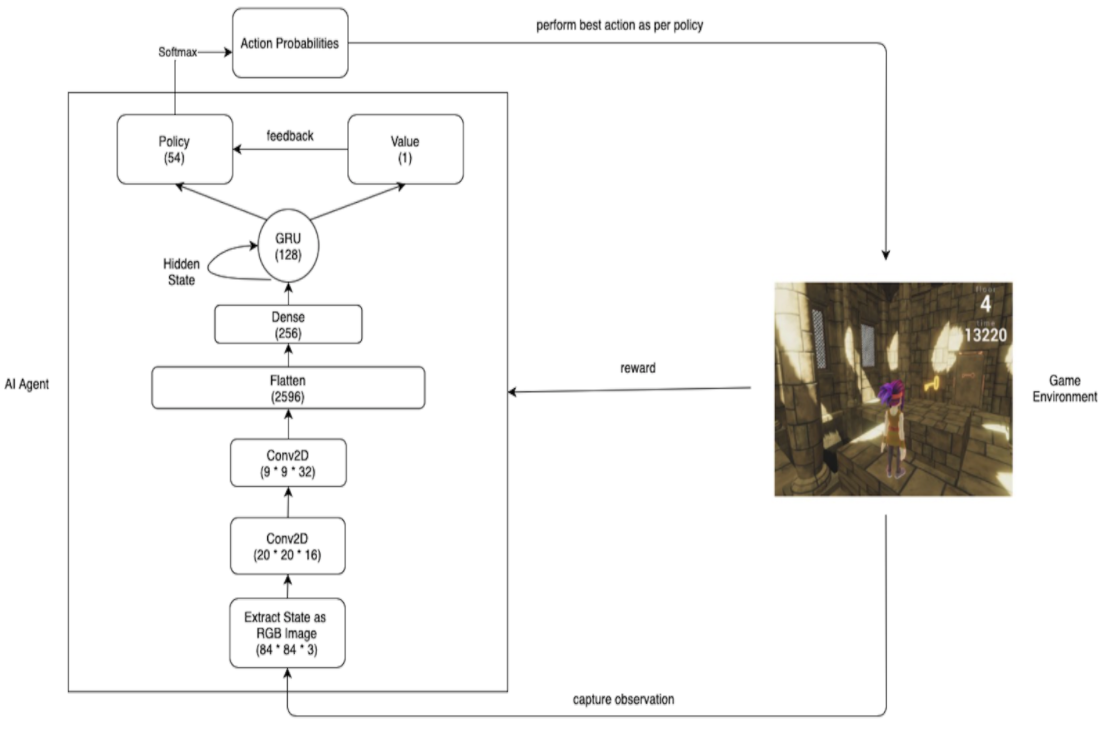
\includegraphics[width=\textwidth]{gameplay.png}
  \caption{Gameplay Setup}
  \label{gameplay_setup}
\end{figure*}

\subsection{\textbf{Asynchronous Advantage Actor Critic (A3C) Model}}
The Asynchronous Advantage Actor Critic (A3C) \cite{Mnih-et-al-2016} algorithm is one of the latest advances in the field of Deep RL. This algorithm was developed by Google’s DeepMind. Here is a breakdown of the different terms in this model:

\begin{itemize}
	\item \textbf{Asynchronous}: Common Deep RL algorithms like Deep Q-Learning use only one agent and one environment. However, in A3C, there are multiple workers with each one operating in its own environment. These workers or agents learn asynchronously with each timestep. As each agent learns, it contributes its total knowledge to the global network and synchronizes with the latest information from it. Worker agents help to see more diversified training data. 

	\item \textbf{Advantage}: It is a formula which uses an approximation of Q-values to estimate the best action that can be performed in any given state by calculating the difference between the best action and the actual action. This results in training the policy to move towards using the best actions.

	\item \textbf{Actor-Critic}: Instead of using one of either policy gradient methods or value iteration methods, the algorithm employs the best of both by predicting the value function \textbf{V} and the optimal policy function $\pi(a_t|s_t; \theta$). The Critic uses value and provides that as a feedback to the Actor which learns the policy and determines a conditional probability distribution of actions, \textbf{P}($a \mid s; \theta$).

\end{itemize}

The formula for policy update is as seen in Fig. \ref{a3c_policy_update}:

\begin{figure}[h]
  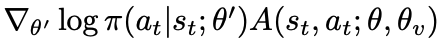
\includegraphics[width=\linewidth]{a3c_loss.png}
  \caption{Policy Update}
  \label{a3c_policy_update}
\end{figure}

The advantage function is approximated by the formula in Fig. \ref{a3c_advantage}. Here, k can vary from state to state and is upper-bounded by $t_{max}$.

\begin{figure}[h]
  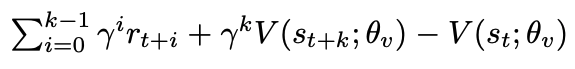
\includegraphics[width=\linewidth]{advantage.png}
  \caption{Advantage Formula}
  \label{a3c_advantage}
\end{figure}

Instead of experience replay, numerous agents work asynchronously as seen in Fig. \ref{a3c_multi_worker}, each with their own environment. Due to the nature of this parallelism, each agent has its own experience of a plethora of states and the data of the agent is decoupled into a stationary process. Therefore, models like SARSA, N-Step methods, and actor critic methods can be applied in a more robust way and neural networks can be utilized more efficiently.

\begin{figure}[h]
    \centering
    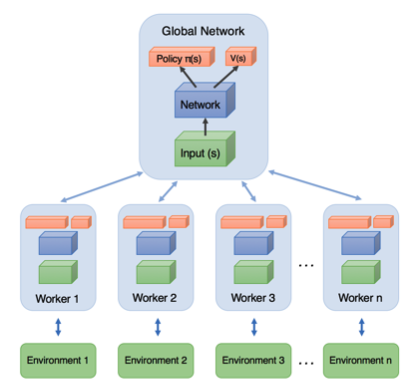
\includegraphics[width=8cm]{a3c_multi_worker.png}
    \caption{Distributed Actor Critic Setup}
    \label{a3c_multi_worker}
\end{figure}

\subsection{\textbf{Policy and Value Network Architectures}}

Network architectures for value and policy are equally important for the performance of our agent. Reinforcement learning implementations use two approaches to implement these networks. One is where there are separate networks for policy and value. In such an implementation, no parameters are shared between the two networks. The second approach uses a single network that is shared for both components which allows the agent to learn faster. 

This project uses the latter implementation. Two different architectures were attempted. A CNN based architecture to capture spatial features from agent’s visual observations. It has 3 convolutional layers and dense layers for predicting policy actions and value. The second model uses a CNN-GRU based architecture to capture both spatial and temporal dependencies. These architectures are detailed in Fig. \ref{a3c_cnn} and Fig. \ref{a3c_cnn_gru} below. 

\begin{figure}[htp]
    \centering
    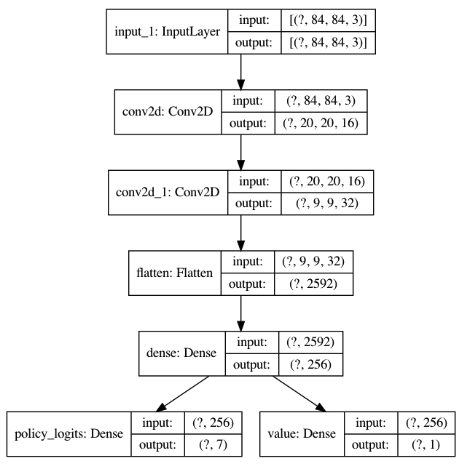
\includegraphics[width=\linewidth]{a3c_cnn.png}
    \caption{A3C - CNN Model}
    \label{a3c_cnn}
\end{figure}

\begin{figure}[htp]
    \centering
    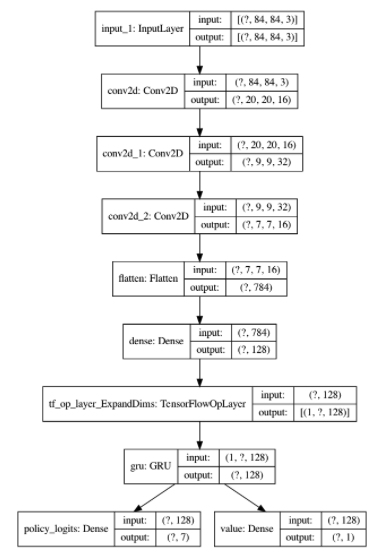
\includegraphics[width=\linewidth]{a3c_gru.png}
    \caption{A3C - CNN+GRU Model}
    \label{a3c_cnn_gru}
\end{figure}

\subsection{\textbf{Proximal Policy Optimization (PPO)}}

Introduced in 2017 by OpenAI, PPO \cite{Open-ai-gym} is an on-policy algorithm that aims to provide faster and smoother training without a significant increase in bias. Since PPO is on-policy, it uses a batch of experiences only once i.e. there is no replay buffer to go over the same experiences again and again. PPO can be incorporated with A3C architecture for the purpose of training agents. 

RL suffers from a problem: training data is directly dependent on the policy since it is the policy that is responsible for taking actions which lead to observations which are then taken as new data. Data distribution over observation and rewards is always changing. This also makes it susceptible to difficulty in hyper-parameter tuning. PPO offers ease of implementation, sample efficiency and ease of tuning.

The heart of PPO is its loss function. The primary field of loss function consists is called a clipped surrogate objective. This consists of two parts:

\begin{enumerate}
  \item \textbf{Default objective for policy gradient}:
    It pushes the objective functions towards regions with high positive advantage over baseline. It consists of two terms.
    \begin{enumerate}
        \item \textbf{R-theta}:
            This is the probability ratio of the current policy and old policy. 
        \item \textbf{Advantage}:
            This estimates the relative value of selected action. 
            \begin{itemize}
                \item If A $>$ 0, our actions yielded better than expected return. So after A exceeds a point, the action has become more probable after the last gradient step, we don’t want to keep updating too much or else it might get worse. Hence clipping works in this case, it limits the effect of gradient update.
                \item If A $<$ 0, out actions yielded worse than expected return. If A $<$ 0, action might become less probable, don’t keep reducing it’s likelihood too much now. Hence clipping works here as well.
            \end{itemize}
            The key thing to remember here is that the advantage function is noisy, so we don’t want to destroy a policy just based on a single estimate.
    \end{enumerate}
  \item \textbf{Clip}: This part consists of a clipped version of the normal policy gradient objective function that constrains the value of policy loss between:
  \[(1\ -\ clip\ threshold,\ 1\ +\ clip\ threshold)\ *\ advantage\]
  It is responsible for discouraging the policy to deviate too much if the algorithm is already converging towards a currently found good policy.
\end{enumerate}

The primary hyper-parameters used by both models have been defined in Table \ref{hyperparam_table}.

\begin{table}[h!]
    \centering
    \begin{tabular}{ |l|l|l|l| } 
        \hline
        Parameter & A3C Model & PPO Model \\
        \hline
        Optimizer              & Adam           & Adam \\ 
        Learning Rate          & 0.001          & 0.0001 \\ 
        Episodes               & 100            & 100 \\ 
        Update Frequency       & 1000 timesteps & 1000 timesteps \\ 
        Discount Factor/ Gamma & 0.99           & 0.99 \\ 
        Value Coefficient      & 0.5            & 0.5 \\ 
        Clipping Threshold     & -              & 0.2 \\
        Entropy Beta           & -              & 0.001 \\
        Lambda                 & -              & 0.95 \\
    \hline
    \end{tabular}
    \vspace{1ex}
    \caption{Implementation hyper-parameters}
    \label{hyperparam_table}
\end{table}

\subsection{\textbf{Implementation Tactics}}

In addition to developing model networks and architectures, implementation level strategies have also been tried to tweak the models to train better and faster.

\begin{enumerate}
    \item \textbf{Action Space Reduction}: Large action spaces lead to large branching factors which leads to poor decision taking abilities in the agent. Fewer actions led to smaller branching factor leading to faster actions and better training decisions. In our implementation, we reduced the action space from 54 to 7. Our approach to choosing actions was to choose only those action combinations that are natural for a human to perform. In addition to this, we also fixed the floor generation seed and set the "visual-theme" parameter to 0. This makes sure that only the default theme is in place thereby removing generalization. 
    \item \textbf{Retro Mode}: Our game comes with a mode called "Retro". In this mode, the supplemental information like number of keys in possession, time remaining and current floor are embedded inside the image. By setting the retro mode to False, the code was refactored to make sure the image is no longer embedded with the data and we receive the data separately as a tuple. This removes the issue of having to use computer vision and OCR to extract the data.
    \item \textbf{Updated Rewards}: Extrinsic rewards were updated to prioritize collection of keys, time orbs and crossing of floors. This trains the agent to focus on these tasks and penalizes it when it performs anything else. The updated extrinsic reward scheme can been seen in Table \ref{reward_table}.
\end{enumerate}

\begin{table}[h!]
    \centering
    \begin{tabular}{ |l|l|l|l| } 
        \hline
        Task & Original Reward & Updated Reward \\
        \hline
        Completing a floor   & +1   & 1 + (rem. time / 10000) \\ 
        Opening a door       & +0.1 & +0.1 \\ 
        Acquiring a key      & +0.1 & +1 \\ 
        Acquiring a time orb & +0.1 & +1 \\ 
        Solving a puzzle     & +0.1 & +0.1 \\ 
        Time runs out        & 0    & -1 \\ 
    \hline
    \end{tabular}
    \vspace{1ex}
    \caption{Reward Shaping}
    \label{reward_table}
\end{table}

\section{Results and Analysis}

We have successfully trained 2 models so far using the A3C and PPO models. Each of the models have been trained for 100 game episodes totalling $\sim70,000$ timesteps.

Looking at the loss graphs in Fig. \ref{a3c_cnn_result} and Fig. \ref{a3c_gru_result}, we learn that since these algorithms are on-policy, they need a huge amount of training to develop a meaningful policy. Although the training done so far is fairly limited, we see a steady improvement in the collected rewards. Spikes in the loss function mean that the algorithm is exploring new trajectories which is consistent with expected results of initial training for the models.

\begin{figure}[h!]
    \centering
    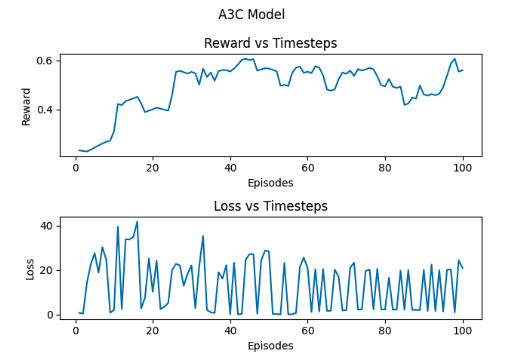
\includegraphics[width=\linewidth]{a3c_cnn_result.png}
    \caption{A3C CNN Model Results}
    \label{a3c_cnn_result}
\end{figure}

\begin{figure}[h!]
    \centering
    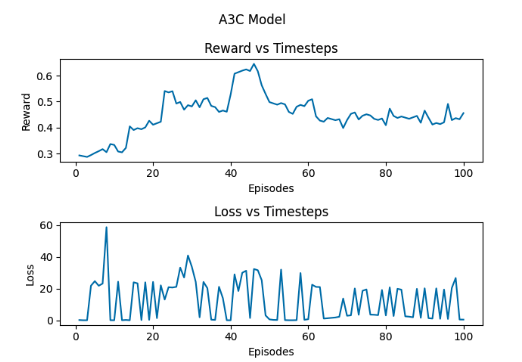
\includegraphics[width=\linewidth]{a3c_gru_result.png}
    \caption{A3C CNN+GRU Model Results}
    \label{a3c_gru_result}
\end{figure}

In the reward graphs for the A3C models, we see a maximum reward of 0.6 which is reached very early in the training period with a gradual degradation later on. As per Fig. \ref{ppo_cnn_result} and Fig. \ref{ppo_gru_result}, the PPO model performs better in terms of registering lower loss values and showing fewer loss spikes. But, the overall score achieved is lesser.

\begin{figure}[h!]
    \centering
    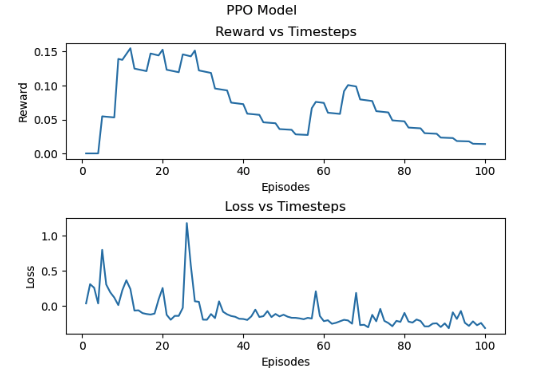
\includegraphics[width=\linewidth]{ppo_cnn_results.png}
    \caption{PPO CNN Model Results}
    \label{ppo_cnn_result}
\end{figure}

\begin{figure}[h!]
    \centering
    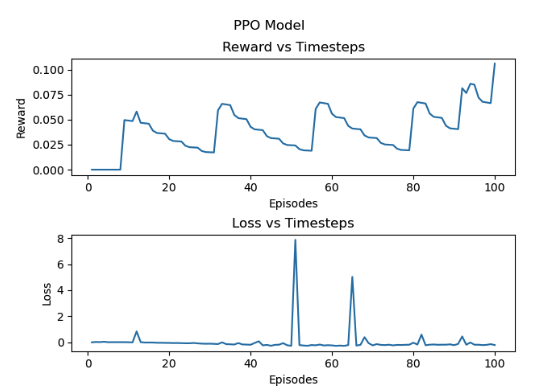
\includegraphics[width=\linewidth]{ppo_gru_results.png}
    \caption{PPO CNN+GRU Model Results}
    \label{ppo_gru_result}
\end{figure}

An interesting insight from the distributed training in Fig. \ref{multi_worker_graph} using thread-based parallelism shows that although we get a significant performance improvement from using multiple workers, as seen in the below graph, we reach optimal performance using 4 workers. This is against the idea that more workers means faster training. A hypothesis behind a decrease after this may be due to the increased inter-thread communication cost that happens during synchronization of weights with the master/global agent network. To put this in perspective, all the workers were created in threads on the same local machine. We expect to achieve better performance with distributed tensorflow which will enable us to employ more than 1 machine.

\begin{figure}[h!]
    \centering
    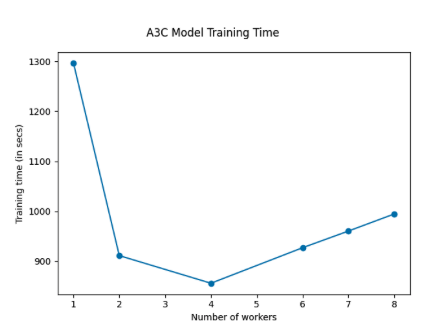
\includegraphics[width=\linewidth]{multi_worker.png}
    \caption{Distributed Model Training}
    \label{multi_worker_graph}
\end{figure}

\section{Limitations}

% Actor-critic methods combine policy gradient methods with a learned value function. With DQN, we only had the learned value function — the Q-function — and the "policy" we followed was simply taking the action that maximized the Q-value at each step. With A3C, as with the rest of actor-critic methods, we learn two different functions: the policy (or "actor"), and the value (the "critic"). The way the policy adjusts the action probabilities relies on the current advantage, which in turn is an estimate. It is important to note that it is also dependent on the value function updates with respect to the experience and rewards collected by following the policy.


% The key to A3C is the parallelized architecture which is also asynchronous by design: plethora of actor-learners are deployed to separate instantiations of the environment; interaction is performed by all these agents, and as stated earlier they asynchronously push the gradients to a central "crucial" network (an idea borrowed from DQN). Surprisingly, Open AI showed that with A2C asynchronicity is not the primary reason for increased performance. In fact, they showed that it reduces sample efficiency.

The drawbacks for A3C and A2C are environments with complex tasks, limited observability, and increased delays between taking an action and receiving some meaningful reward. Naturally, researchers have pondered on this idea and several sub-fields in the domain of reinforcement learning have emerged.

% Open AI introduced PPO in 2017 and within no time, it has risen to become the most popular reinforcement learning algorithm overtaking Deep-Q learning. The way it approaches the problem is unique and profound. It starts of by collecting a mini batch of experiences interacting with the environment around the agent. Next, it uses a batch-update to update its decision-making policy. These batches are disposed immediately after the policy is updated, and a fresh batch is collected next. This forms the critical part of why it is an "on-policy learning" approach because similar to other "on-line gradient-descent"  algorithms, the metric, here the policy, gets update frequently in the form a stream.

% Moreover, the differences between the updated policy, and immediate-previous-policy is not very significant. This means less variance in training. However, we will still incur the cost of some bias. Nevertheless, we get a smoother training and we can ensure that the agent does not go down a path which is unrecoverable.

There are methods such as policy gradient methods which are less sample efficient than Q-learning. This is because you only use the data once after which it is discarded.

The way reinforcement learning models the problem requires several conditions:
\begin{enumerate}
    \item \textbf{Ability to quantify all the variables of the environment}: In the real world, it is natural to expect that we have access to either partial or no information. Information might also be inaccurate.

    \item \textbf{Mathematical expression of reward}: How can we distinguish between good reward and bad reward? Formulating rewards to enable meaningful learning is seldom observed in human learning experiences.

    \item \textbf{Simulation}: Learning environments have the luxury to have commit mistakes indefinitely without negative consequences. This is not so in real life.
    
    \item \textbf{Increased training time}: This is fine if the task under consideration is simple and easy to solve, actions are discrete, and the information present is immediately available. Sometimes, problem formulation is so complex that we must balance the precision of our simulator with both training time and real-time performance constraints.
    
    \item \textbf{High data requirement}: This is equivalent to thousands of computing hours in a simulator. This is needed to match human level performance even in trivial tasks. For example, Rainbow DQN plays a number of games with the same engine and picks the best algorithm as a comparison. Such an algorithm requires 44 million frames to learn to play with superhuman capabilities. Rainbow DQN passes the 100\% threshold (just above human capabilities) at about 18 million frames. In other words, this is about 83 hours of the play experience. To this number, one should add the time for training the model.
    
    \item \textbf{Discrete action spaces}: In many real use cases, agents perform actions in a continuous space. Making a discrete action continuous is not only non-trivial but will also increase the number of (discrete) actions the agent will have to deal with during policy optimization. This, in turn, affects training time and performance.
    
    \item \textbf{Local Optima}: It is easier for agents to get stuck in local minima. 
\end{enumerate}

\section{Future Work}

\subsection{\textbf{Curiosity based learning}}

One of the biggest challenges to RL algorithms is the problem of sparse rewards. Most external rewards that an agent gets from the environment are extremely sparse. This leads to difficulty in training where the agent has to try a huge number of trajectories before it finally finds a one that it can converge on. This leads to training time overhead. Some methods to counter this issue use tricks like reward shaping which only work well for specific environments. Most agents trained using reward shaping do not generalise well to new levels/tasks. 

Curiosity provides an intrinsic reward signal that helps agents explore the environment. Pathak-et-al \cite{Pathak-et-al} defines curiosity as “an error in the agent’s ability to predict the consequence of its own actions”. Their curiosity formulation helps the agent take into account things that affect it and ignore the ones that do not. They investigated three curiosity categories:

No extrinsic reward: the agent trained on curiosity is able to explore the environment better
Generalization: the agent trained on other levels of the games is asked to play a completely unseen level. The idea is for the agent to be able to use its previous experiences to explore the environment better


\begin{itemize}
\item Sparse extrinsic reward: the agent trained on curiosity takes fewer steps to reach the goal
\item No extrinsic reward: the agent trained on curiosity is able to explore the environment better
\item Generalization: the agent trained on other levels of the games is asked to play a completely unseen level.
The idea is for the agent to be able to use its previous experiences to explore the environment better
\end{itemize}

\subsection{\textbf{Distributed Tensorflow}}

Using distributed training, we can train very large models and speed up training time. Tensorflow provides a high-end API to train your models in a distributed way with minimal code changes.  Two types of paradigms used for distributed training:
Data Parallelism: Models are replicated into different devices (GPU) and trained on batches of data.
Model Parallelism: Models are too large to fit on a single device and are distributed over many devices.
We will be investigating utilization of distributed tensorflow so that we can train our agents faster and tighten the developer feedback loop.

\subsection{\textbf{IMPALA}}

IMPALA \cite{Espeholt-et-al} is an efficient and quick way of performing a huge number of tasks with only one reinforcement learning agent and only one set of parameters. By handling resources more efficiently in  single machine training, IMPALA can be extended to work on multiple machines without jeopardizing data efficiency. With the use of an off-policy correction method called V-trace together with disjoint acting and learning, consistent learning at high throughput is achieved.

Without compromising on training stability and data efficiency, IMPALA can scale to thousands of machines. Instead of communicating gradients with the learners as in A3C, the workers send a tuple(state sequence, action, rewards) to a centralized learner. A GPU is used to perform updates on small batches of these tuples or rather trajectories, and simultaneously parallely perform all operations that do not depend on other operations; this is because the learner is the one with complete access to all such tuples. Due to this decoupled architecture, IMPALA is known to have great efficiency. The only challenge in this algorithm is to make sure that the trajectory generation policy is not lagging behind the learner in terms of the updates when the gradient is being calibrated. Therefore the learning becomes off policy. To appropriately resolve this discrepancy,  V-trace off-policy actor-critic algorithm comes into the picture. Below is a picture of the formula for V-trace.

\subsection{\textbf{Longer Training}}
Most of the competitors and the winners of Obstacle Tower Challenge have trained for significantly longer timesteps to obtain optimal results for the agent. In the remaining half of the semester our goal is to reach 5 million timesteps for training.

\section{Conclusions}

As is evident from the discussion, our agent currently is able to take actions that allow it to progress in the game. However, these are still early days, and with the introduction of distributed training, IMPALA, Curiosity-based learning, etc, our agent will be able to take many optimal decisions and we are expecting it to go past several levels in the Obstacle Tower.

\section{Acknowledgement}

We would like to thank Professor Dr. Michael Zyda and the TA's for allowing us to work on this project.

\begin{thebibliography}{00}
\bibitem{Juliani-et-al} Juliani, Arthur \& Khalifa, Ahmed \& Berges, Vincent-Pierre \& Harper, Jonathan \& Teng, Ervin \& Henry, Hunter \& Crespi, Adam \& Togelius, Julian \& Lange, Danny. (2019). Obstacle Tower: A Generalization Challenge in Vision, Control, and Planning. 2684-2691. 10.24963/ijcai.2019/373.
\bibitem{Bellemare-et-al} Bellemare, Marc \& Naddaf, Yavar \& Veness, Joel \& Bowling, Michael. (2012). The Arcade Learning Environment: An Evaluation Platform for General Agents. Journal of Artificial Intelligence Research. 47. 10.1613/jair.3912.
\bibitem{Mnih-2015} Mnih, Volodymyr et al. (2015). Human-level control through deep reinforcement learning. Nature. 518. 529-33. 10.1038/nature14236.
\bibitem{Unity-tech-blog} “Announcing the Obstacle Tower Challenge Winners and Open Source Release.” Unity Technologies Blog, Unity Technologies, 14 Aug. 2019, blogs.unity3d.com/2019/08/07/announcing-the-obstacle-tower-challenge-winners-and-open-source-release/.
\bibitem{Pickled-ml-blog} "Competing in the Obstacle Tower Challenge" Pickled-ml-blog, Freelancer blog, 24 Jul. 2019, blog.aqnichol.com/2019/07/24/competing-in-the-obstacle-tower-challenge/
\bibitem{Zhang-et-al} Zhang, Hongyi, Yann N. Dauphin, and Tengyu Ma. "Fixup initialization: Residual learning without normalization." arXiv preprint arXiv:1901.09321 (2019).
\bibitem{Berthelot} Berthelot, David, Nicholas Carlini, Ian Goodfellow, Nicolas Papernot, Avital Oliver, and Colin Raffel. "Mixmatch: A holistic approach to semi-supervised learning." arXiv preprint arXiv:1905.02249 (2019).
\bibitem{Unity_ml_agents_tech_blog} "Unity Machine Learning Agents" Unity Technologies Blog, Unity Technologies, 1 Jan. 2021, unity.com/products/machine-learning-agents
\bibitem{Open-ai-gym} "Open-ai-gym" Open AI Blog, Open AI, 1 Jan. 2021, gym.openai.com
\bibitem{Sokoban} "Sokoban" Wikipedia website, Wikipedia, 26 Feb. 2021, en.wikipedia.org/wiki/Sokoban
\bibitem{Mnih-et-al-2016} Mnih, Volodymyr, Adria Puigdomenech Badia, Mehdi Mirza, Alex Graves, Timothy Lillicrap, Tim Harley, David Silver, and Koray Kavukcuoglu. "Asynchronous methods for deep reinforcement learning." In International conference on machine learning, pp. 1928-1937. PMLR, 2016.
\bibitem{Schulman-et-al} Schulman, John \& Wolski, Filip \& Dhariwal, Prafulla \& Radford, Alec \& Klimov, Oleg. (2017). Proximal Policy Optimization Algorithms.
\bibitem{Pathak-et-al} Pathak, Deepak, Pulkit Agrawal, Alexei A. Efros, and Trevor Darrell. "Curiosity-driven exploration by self-supervised prediction." In International Conference on Machine Learning, pp. 2778-2787. PMLR, 2017.
\bibitem{Espeholt-et-al} Espeholt, Lasse \& Soyer, Hubert \& Munos, Remi \& Simonyan, Karen \& Mnih, Volodymir \& Ward, Tom \& Doron, Yotam \& Firoiu, Vlad \& Harley, Tim \& Dunning, Iain \& Legg, Shane \& Kavukcuoglu, Koray. (2018). IMPALA: Scalable Distributed Deep-RL with Importance Weighted Actor-Learner Architectures.
\end{thebibliography}
\vspace{12pt}

\end{document}
